%% Beispiel-Präsentation mit LaTeX Beamer im KIT-Design
%% entsprechend den Gestaltungsrichtlinien vom 1. August 2020
%%
%% Siehe https://sdqweb.ipd.kit.edu/wiki/Dokumentvorlagen

%% Beispiel-Präsentation
\documentclass[en]{sdqbeamer} 

%% Footnote without numbering
\newcommand\nonumberfootnote[1]{%
  \begingroup
  \renewcommand\thefootnote{}\footnote{#1}%
  \addtocounter{footnote}{-1}%
  \endgroup
}
 
%% Titelbild
\titleimage{banner_2020_kit}

%% Gruppenlogo
\grouplogo{} 

%% Gruppenname und Breite (Standard: 50 mm)
\groupname{Institute for Automation and Applied Informatics (IAI)}
%\groupnamewidth{50mm}

% Beginn der Präsentation

\title[ABAC for Substations]{Attribute-Based Access Control for Substations (ABAC-SS)}
\subtitle{Master's Thesis Proposal} 
\author[Moritz Gstuer]{Moritz Gstuer}

\date[06.\,06.\,2024]{06. June 2024}

% Literatur 
 
\usepackage[citestyle=authoryear,bibstyle=numeric,hyperref,backend=biber]{biblatex}
\addbibresource{../bibliography/masterthesis.bib}
\bibhang1em

\begin{document}
 
%Titelseite
\KITtitleframe

%Inhaltsverzeichnis
\begin{frame}{Agenda}
\tableofcontents
\end{frame}

\section{Motivation}
\begin{frame}{Motivation}
    \centering
	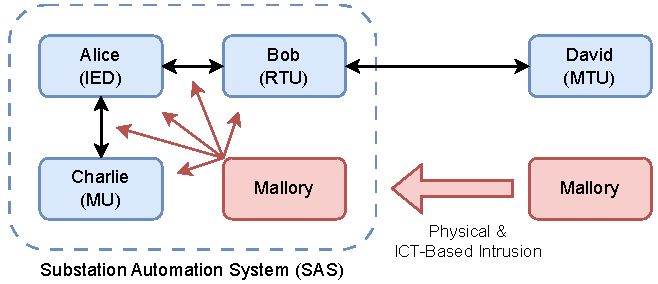
\includegraphics[width=0.8\textwidth]{./figures/sas_intrusion.drawio.pdf}
    \nonumberfootnote{IED\dots Intelligent Electronic Device | MU\dots Merging Unit | RTU\dots Remote Terminal Unit}
    \nonumberfootnote{MTU\dots Master Terminal Unit | ICT\dots Information and Communications Technology}
\end{frame}
\begin{frame}{Motivation}
    \begin{columns}
        \column{.4\textwidth}
        \centering
        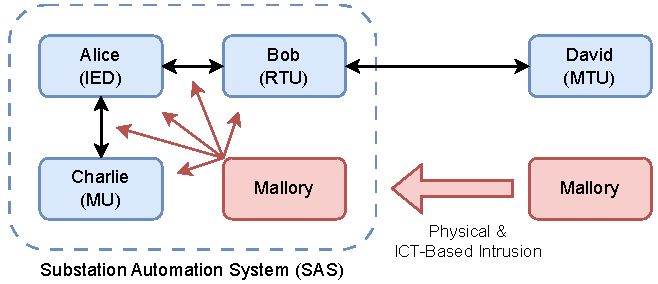
\includegraphics[width=1.0\textwidth]{./figures/sas_intrusion.drawio.pdf}
        \column{.6\textwidth}
        \begin{redblock}{Substation Threats \& Attacks}
            \begin{itemize}
                \item Eavesdropping
                \item Man-in-the-Middle
                \item Spoofing/Masquerading
                \item Replay
                \item Denial of Service\\$\rightarrow$ Flooding, Broadcast/Multicast Storm, \& Poisoning
                \item False Data Injection\\$\rightarrow$ Forged Sensor Data \& Commands, \& Configuration Tampering
            \end{itemize}
            % $\rightarrow$ Authentication, Authorization, Access Control, \& Encryption of Substation Communication
        \end{redblock}
    \end{columns}
\end{frame}

\section{System Model}
\begin{frame}{Substation Automation System (SAS)}
    \centering
	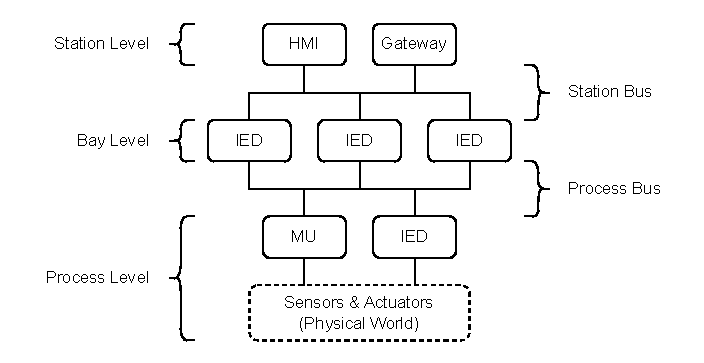
\includegraphics[width=0.7\textwidth]{./figures/substation_architecture.drawio.pdf}
    \nonumberfootnote{IED\dots Intelligent Electronic Device | MU\dots Merging Unit | HMI\dots Human-Machine Interface}
\end{frame}

\begin{frame}{SAS Communication}
    \begin{blueblock}{Station Bus}
        Transport Layer-Based Session-Oriented Communication (e.g. MMS Protocol)
        \\$\rightarrow$ Client-Server (Unicast)
    \end{blueblock}
    \begin{blueblock}{Process Bus}
        Data Link Layer-Based Message-Oriented Communication (e.g. GOOSE \& SV Protocol)
        \\$\rightarrow$ Publisher-Subscriber (Broadcast/Multicast)
    \end{blueblock}
    \begin{grayblock}{IEC 61850 Message Types \& Performance Classes \parencite*{IEC61850P5,IEC61850P8}}
        Requirements for messages in substations
        \\Examples: GOOSE (Type 1A, 3 ms), SV (Type 4, 3 ms), MMS (Type 2/3/5, 100-10000 ms)
    \end{grayblock}
\end{frame}

\begin{frame}{Requirements \& Constraints}
    \begin{columns}
        \column{.5\textwidth}
        \begin{blueblock}{Security}
            \begin{itemize}
                \item Confidentiality
                \item Integrity
                \item Authenticity
                \item Non-Repudiation
                \item Least Privilege Principle (PoLP)
                \item Separation of Duties (SoD)
                \item Privacy-Preservation
            \end{itemize}
            $\rightarrow$ Encryption, Authentication, \& Authorization
        \end{blueblock}
        \column{.5\textwidth}
        \begin{blueblock}{Performance}
            \begin{itemize}
                \item Soft \& Firm Real-Time
                \item CPU \& Memory
                \item Energy \& Power
            \end{itemize}
            $\rightarrow$ Separation of Concerns \& Modularity
        \end{blueblock}
        \begin{blueblock}{Interoperability}
             Existing Inter-/Intra-SAS Protocols \& SCADA Systems
             \\$\rightarrow$ Compatibility \& Interchangeability
        \end{blueblock}
    \end{columns}
\end{frame}
\begin{frame}{Requirements \& Constraints}
    \begin{redblock}{Overarching Requirements for Operational Technology (OT)}
        \begin{itemize}
            \item Availability
            \item Safety
        \end{itemize}
        Under any Circumstances: Continuing \& Safe Operation
        \\$\rightarrow$ Fail-Operational (before Fail-Safe)
    \end{redblock}
\end{frame}

\section{Related Work}
\begin{frame}{Related Work}
    \begin{blueblock}{IEC 62351 \parencite*{IEC62351P6,IEC62351P8}}
        Standard for Cybersecurity: Energy-Related Systems \& Communication Networks
        \\$\rightarrow$ Authenticity \& Integrity: Mandatory Symmetric Authentication
        \\$\rightarrow$ Confidentiality: Optional (Non-Recommended) Symmetric Encryption
        \\$\rightarrow$ Access Control: Role-Based Access Control (RBAC) (Access-Token-Driven, 7 Mandatory Roles)
    \end{blueblock}
\end{frame}
\begin{frame}{Related Work}
    \begin{blueblock}{Secure Communication in Substations}
        \begin{itemize}
            \item Bump-in-the-Wire Security Filter for GOOSE/SV MAC Tagging \& Verification \parencite{Ishchenko2018}
            \item Domain-Based Collaborative Cyberattack Mitigation Approach \parencite{Hong2019}
            \item Fixed-Latency Hardware Architecture for GOOSE/SV Encryption \& Authentication \parencite{Rodriguez2021}
        \end{itemize}
    \end{blueblock}

    \begin{blueblock}{Role-Based Access Control (RBAC) in Substations}
        \begin{itemize}
            \item XACML-Based RBAC Approach for IEC 61850 \& IEC 62351 compliant SAS \parencite{Lee2015}
            \item Distributed RBAC for Subscription-Based Remote Network Services \parencite{Ma2006} % Constraint-Enabled 
            \item Rule-Based RBAC Policy Enforcement Architecture \parencite{Alcaraz2016} % for Smart Grid Systems
        \end{itemize}
    \end{blueblock}
\end{frame}
\begin{frame}{Related Work}
    \begin{blueblock}{Attribute-Based Access Control (ABAC) in Substations}
        \begin{itemize}
            \item Firewall for Attribute-Based Access Control in Smart Grids \parencite{Ruland2018}
            \\$\rightarrow$ Firewall with XACML-Based ABAC Policies
            \\$\rightarrow$ Outer \& Inner Station Bus
            \\$\rightarrow$ Unobstructed Fast Messages (e.g. GOOSE)
            \item T-ABAC: An attribute-based access control model for real-time availability in highly dynamic systems \parencite{Burmester2013}
            \\$\rightarrow$ Real-Time Attribute Values
            \\$\rightarrow$ Labeling of High Priority Packets
            \\$\rightarrow$ Domain-Based Congestion Avoidance
        \end{itemize}
    \end{blueblock}
    % Message Authentication, Asym. Performance Evaluation, BitW- \& HW-Solutions, Access Control
\end{frame}

\begin{frame}{Research Questions}
    \begin{greenblock}{Attribute-Based Access Control in Substations}
        How can ABAC approaches be employed to secure modern SAS?
        \\$\rightarrow$ Real-Time Attributes, Ad-Hoc Policy Evaluation, \& Speedup Solutions
    \end{greenblock}

    \begin{greenblock}{Confidentiality, Integrity, \& Authenticity of Communication in Substations}
        Which cryptographic techniques are suitable for securing internal \& external communication of a SAS?
        \\$\rightarrow$ Asymmetric/Symmetric Cryptography, (Dis-)Advantages, Speedup Solutions, \& Resource Constrained Devices
    \end{greenblock}

    \begin{greenblock}{Substation Security Framework for Time-Critical Communication}
        How can authentication, authorization, access control, \& encryption be integrated into a security framework which is able to secure time-critical SAS communication?
        \\$\rightarrow$ System Model, Domain Requirements, Architecture, \& Protocols
    \end{greenblock}
\end{frame}

\section{Proposed Approach: SAZE}
\begin{frame}{SAZE ("Sassy") Approach}
    \begin{greenblock}{\textbf{S}erver-aided \textbf{A}BAC with \textbf{Z}ero-RTT \textbf{E}ncryption (SAZE)}
        \begin{itemize}
            \item Mandatory Access Control \& Encryption for SAS Communication
            \item Transparent Security for SAS Devices (e.g. IED \& MU)
        \end{itemize}
    \end{greenblock}
    %Overview: Describe parts Server-Aided Attribute-Based Access Control (Including Authentication and Authorization Delegation) with Zero-RTT Encryption (Asym./Sym.)
\end{frame}

\begin{frame}{SAZE Components}
    \centering
	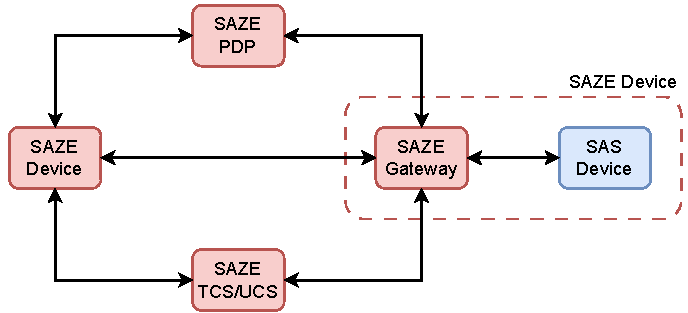
\includegraphics[width=0.75\textwidth]{./figures/saze_components_color.drawio.pdf}
    \nonumberfootnote{PDP\dots Policy Decision Point | TCS/UCS\dots Trusted/Untrusted Cryptography Server | SAS\dots Substation Automation System}
\end{frame}

\begin{frame}{SAZE SAS Architecture}
    \begin{columns}
        \column{.7\textwidth}
        \centering
        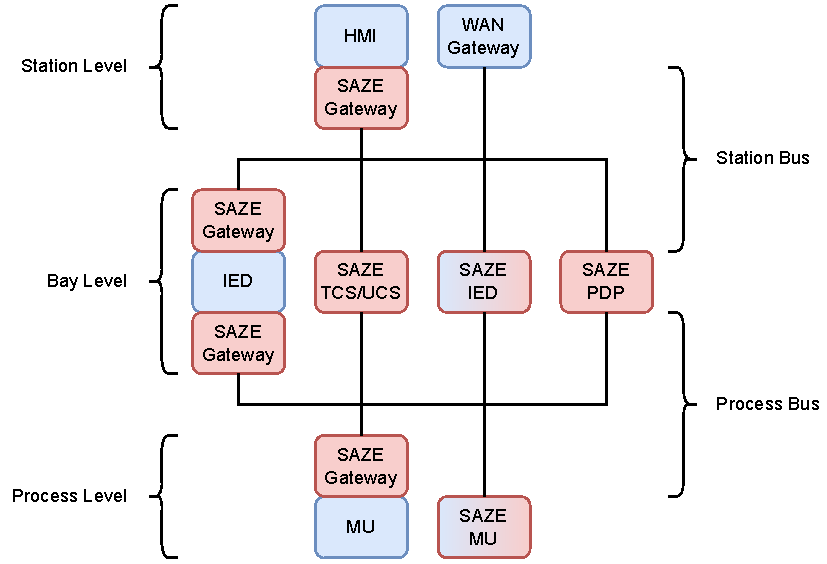
\includegraphics[height=0.75\textheight]{./figures/saze_architecture_color.drawio.pdf}
        \column{.3\textwidth}
        \footnotesize
        HMI\dots Human-Machine Interface\\IED\dots Intelligent Electronic Device\\MU\dots Merging Unit\\PDP\dots Policy Decision Point\\TCS\dots Trusted Cryptography Server\\UCS\dots Untrusted Cryptography Server\\WAN\dots Wide Area Network
    \end{columns}
\end{frame}

\subsection{Server-Aided ABAC}
\begin{frame}{Attribute-Based Access Control (ABAC)}
    \begin{greenblock}{Definition \parencite{JTF2020}}
        Access control model enabling access decisions based on attributes associated with \textbf{subjects}, \textbf{objects}, \textbf{actions}, and the \textbf{environment} of a system.
    \end{greenblock}

    \begin{blueblock}{Discussion \parencite{Hu2014}}
        \begin{itemize}
            \item Multifactor Policy Expression $\rightarrow$ Fine-Grained \& Flexible Access Control (cf. RBAC/IBAC)
            \item Dynamic Policy Evaluation $\rightarrow$ Dynamic Authorization \& Real-Time Attributes
        \end{itemize}
    \end{blueblock}

    \begin{grayblock}{Architecture \parencite{Hu2014,Oasis2013}}
        \begin{itemize}
            \item Policy Decision Point (PDP) $\rightarrow$ Computes access decisions by evaluating policies
            \item Policy Enforcement Point (PEP) $\rightarrow$ Enforces policy decisions by controlling access to protected objects
        \end{itemize}
    \end{grayblock}
    % ABAC Definition
    % ABAC Benefit vs. traditional IBAC/RBAC solutions including RT-Attribute like network congestion
    % ABAC Requirements -> Authentication \& Authorization
\end{frame}

\begin{frame}{Authorization, Authentication, \& Access Control}
    \centering
	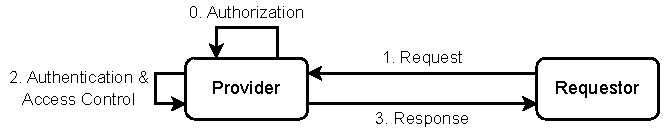
\includegraphics[width=0.9\textwidth]{./figures/access_control_request_traditional.drawio.pdf}
    \begin{redblock}{Problem}
        Too many provider responsibilities
        \\$\rightarrow$ Policy Management/Decisions/Enforcement, Request Verification, \& Response Creation
    \end{redblock}
\end{frame}

\begin{frame}{Server-Aided ABAC}
    \begin{redblock}{Problem: Policy Evaluation Complexity}
        Fine-grained \& flexible access control relying on dynamic authorization \& ad-hoc evaluation
        \\$\rightarrow$ Complex policy evaluation in real-time environment
    \end{redblock}

    \begin{greenblock}{Solution: Server-Aided ABAC}
        Delegation of authentication, authorization, \& access control to semi-trusted server (PDP)
        \\$\rightarrow$ Evaluates policies \& makes access decisions on request
        \\$\rightarrow$ Speedup Techniques: Evaluation Pre-Computation \& Access Decision Caching
    \end{greenblock}
    % ABAC Problem -> Performance/Computational Effort/Certificates for Attributes\dots
    % Idea -> Authentication and Authorization Delegation to Server => "Server-Aided ABAC"
\end{frame}

\begin{frame}{Server-Aided ABAC}
    \centering
    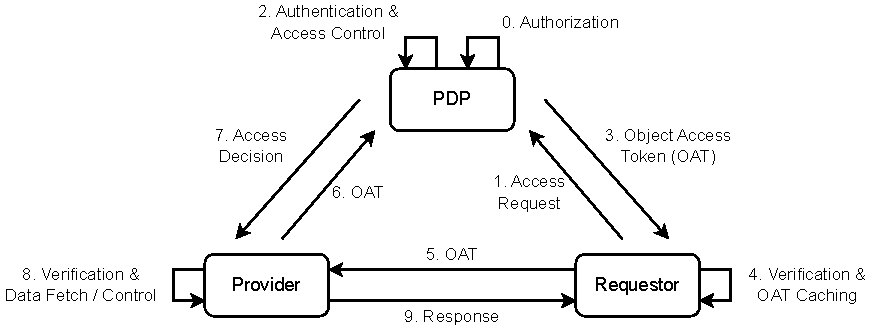
\includegraphics[width=1.0\textwidth]{./figures/access_control_request_delegation.drawio.pdf}
\end{frame}

\subsection{Zero-RTT Encryption}
\begin{frame}{Zero-RTT Encryption}
    \begin{greenblock}{Concept}
        Encrypted communication without prior session/connection handshake
        \\$\rightarrow$ Communication with Zero Round-Trip-Time (Zero-RTT) Handshake
    \end{greenblock}

    \begin{blueblock}{Discussion}
        \begin{itemize}
            \item Initialization Latency: Zero-RTT
            \item Communication Latency: Cryptography \& Transmission Overhead
        \end{itemize}
        $\rightarrow$ Problem: Non-Cacheable Authorizations \& Message-Based Ethernet Communication
    \end{blueblock}
    % Problem: Enc. in substation -> Initialization vs. Communication Latency
    % Init Latency: Solvable via Zero-RTT solution -> Not straight forward because Ethernet-Based Communication Message-Based not Session-Based
    % -> Not applicable to non-cacheable authorizations
    % Communication Latency: Overhead for Message encryption, transmission etc.
\end{frame}

\begin{frame}{Asymmetric Cryptography in SAS}
    \begin{greenblock}{Advantage: Key Distribution \& Identity Verification}
        Unsecure Network \& Untrusted Network Participants
        \\$\rightarrow$ Easy \& Secure Key Distribution
        % No confidential key material transmitted over unsecure channel
    \end{greenblock}
    \begin{redblock}{Disadvantage: Computational Complexity \parencite{Elbez2019,Ishchenko2018}}
        Example: 1024-Bit RSA Digital Signature vs. 128-Bit HMAC/GMAC
        \\$\rightarrow$ 10 ms vs. 50 µs on RPi2 (1 GHz quad-core)
        \\$\rightarrow$ 0.3 ms vs. 4 µs on Xeon X3440 (2.53 GHz quad-core) 
    \end{redblock}
    \begin{redblock}{Disadvantage: Ethernet-Based Multicast Communication in SAS}
        Message encryption at publisher requires shared private keys for subscribers.
        \\$\rightarrow$ Alternative: Transform unsecure multicast into secure unicast messages
    \end{redblock}
    % Performance Remarks
    % Problem: Solid foundation for approach/framework but too much effort for low performance devices like MUs/IEDs/RTUs
    % Problem 2: Ethernet-based broadcast communication to multiple devices
\end{frame}

\begin{frame}{TLS-Inspired Cipher Change (Alternative 1)}
    \centering
    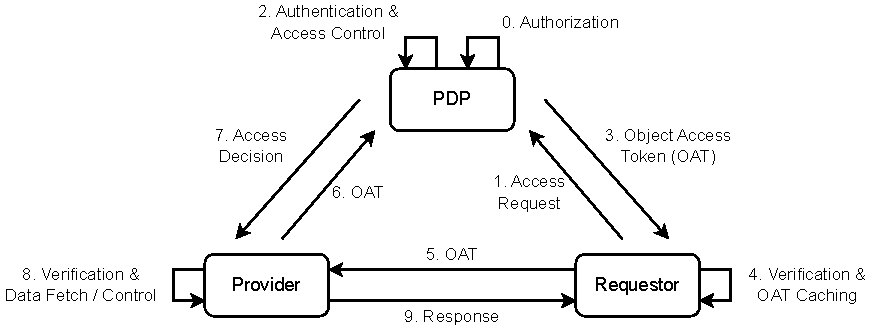
\includegraphics[width=0.5\textwidth]{./figures/access_control_request_delegation.drawio.pdf}
    \begin{greenblock}{Cipher Change Approach}
        Exchange Algorithm \& Key Exchange Parameters \dots
        \begin{itemize}
            \item Directly (5. \& 9. Step)
            \item Indirectly via PDP (1., 7., \& 9. Step)
        \end{itemize}
        $\rightarrow$ Mandatory Asymmetric Cryptography: Only Steps 0-9
    \end{greenblock}
    % Figure with 2 nodes and PDP where initial OAT exchange is also DH key exchange/cipher change
\end{frame}

\begin{frame}{Server-Aided Asymmetric Cryptography (Alternative 2)}
    \begin{greenblock}{Trusted/Untrusted Cryptography Server (TCS/UCS)}
        Provides cryptography services to resource-constrained devices
    \end{greenblock}
    \begin{blueblock}{TCS/UCS Services}
        \begin{itemize}
            \item Server-Aided Verification (SAV) \parencite{Girault2005}
            \item Proxy Re-Encryption (PRE) \parencite{Green2007}
            \item Hardware-Based Cryptographic Accelerator
        \end{itemize}
    \end{blueblock}
    % Optional Untrusted Server-Aided Signing/Verifikation Encryption/Decryption Server
    % Figure with 2 nodes, PDP, and CryptoHelper
\end{frame}

\section{Evaluation}
\begin{frame}{Evaluation: Areas \& Metrics}
    \begin{greenblock}{Security Evaluation}
        Does SAZE provide security against typical substation adversaries \& attacks?
        \\$\rightarrow$ Required Assumptions \& Satisfied Security Requirements/Goals
    \end{greenblock}
    \begin{greenblock}{Performance Evaluation}
        Is SAZE capable of securing low latency communication in substations?
        \\$\rightarrow$ Computational Complexity, Congestion Resistance, \& Supported Message Types
    \end{greenblock}
    \begin{greenblock}{Economic Evaluation}
        Is SAZE an economically feasible solution for the construction or retrofitting of substations?
        \\$\rightarrow$ Retrofitting Capability, Costs, \& Compatibility with Standards
    \end{greenblock}
    % Econ, Perf, Security
\end{frame}

\begin{frame}{Evaluation: SAS Network Testbed}
    \centering
    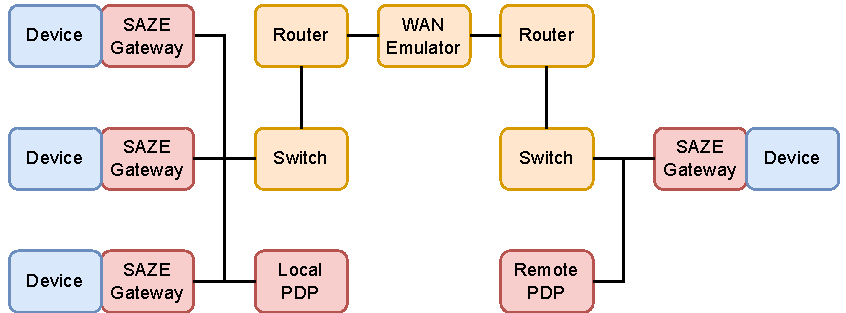
\includegraphics[width=0.7\textwidth]{./figures/network_testbed_color.drawio.pdf}
    \begin{blueblock}{Discussion}
        Results $\rightarrow$ Realistic \& Practice-Oriented 
        \\Repeatability \& Reproducibility $\rightarrow$ Difficult
    \end{blueblock}
    % 2 Possible Implementations
    % Prototype Network (Testbed) with Raspberry Pi using real equipment or simulate SAS traffic -> Figure
    % Network Simulation
\end{frame}

\begin{frame}{Evaluation: Network Simulation}
    \begin{greenblock}{Approach}
        Implementation of SAZE Protocols in Network Simulator
        \\$\rightarrow$ Based on existing protocol implementations for simulators (Ethernet, TCP/IP, GOOSE, SV, MMS\dots)
    \end{greenblock}
    \begin{blueblock}{Discussion}
        Results $\rightarrow$ Uncomparable with SAS
        \\Repeatability \& Reproducibility $\rightarrow$ Easy
    \end{blueblock}
    % 2 Possible Implementations
    % Prototype Network (Testbed) with Raspberry Pi using real equipment or simulate SAS traffic -> Figure
    % Network Simulation
\end{frame}

\section{Conclusion}
\begin{frame}{Conclusion}
    \begin{redblock}{Problem}
        Current ICT-based cyberattack mitigation approaches do not fully cover common attacks on SAS.
        \\Example: Reconnaissance via eavesdropping $\rightarrow$ Confidentiality
        \\Example: Flooding $\rightarrow$ Dynamic authorization based on time-variable attributes
    \end{redblock}
    \begin{greenblock}{Idea}
        Mandatory authentication, authorization, access control, \& encryption of SAS communication
    \end{greenblock}
    \begin{blueblock}{Contribution}
        SAZE security framework\dots
        \\\dots employs mandatory authentication, authorization, access control, \& encryption
        \\\dots for time-critical SAS communication
        \\\dots in time-variable SAS environment.
    \end{blueblock}
\end{frame}

\appendix
\beginbackup

\begin{frame}[allowframebreaks]{References}
\printbibliography
\end{frame}

\backupend

\end{document}